\documentclass[a4paper]{article}
\usepackage[warn]{mathtext}
\usepackage[utf8]{inputenc}
\usepackage[T2A]{fontenc}
\usepackage[english,russian]{babel}
\usepackage{indentfirst}
\usepackage{misccorr}
\usepackage{subcaption}
\captionsetup{compatibility=false}
\usepackage{geometry}
\geometry{verbose,a4paper,tmargin=2cm,bmargin=2cm,lmargin=1.5cm,rmargin=1.5cm}
\usepackage{graphicx}
\usepackage{wrapfig}
\usepackage{amsmath}
\usepackage{fancyhdr}
\usepackage{floatflt}
\usepackage{float}
\usepackage{amssymb}
\usepackage{color}
\usepackage{lscape}
\usepackage{hvfloat}
\usepackage{amsfonts}
\usepackage{euscript}
\usepackage{newunicodechar}
\usepackage{booktabs}



\begin{document}
\newcommand{\apple}{\char"F8FF}

\begin{titlepage}
	\centering
	\vspace{5cm}
    {\scshape\LARGE Московский физико-технический институт\par}


	\vspace{3cm}
	{\scshape\Large Лабораторная работа по общей физике \par}
	\vspace{1cm}
	{\huge\bfseries  1.2 Эффект Комптона \par}
	\vspace{1cm}
	\vfill
\begin{flushright}
	{\large выполнила студентка Б01-907 группы}\par
	\vspace{0.3cm}
	{\LARGE Юлия Прохорова }
\end{flushright}
	
	\vfill
Долгопрудный, 2021
% Bottom of the page
\end{titlepage}

\tableofcontents

\newpage

\section{Цель работы}
\begin{itemize}
    \item С помощью сцинтилляционного спектрометра исследовать энергетическйи спектр
    $\gamma$-квантов, рассеяных на графите
    \item Определяить энергию рассеяных $\gamma$-квантов в зависимости от угла рассеяния
    \item Определить энергию покоя частиц, на которых происходит комптоновское рассеяние
\end{itemize}

\section{Оборудование}
ЭВМ, ФЭУ, cцинилляционный счетчик, графитовая мишень, источник излучения.

\section{Теория}

\textbf{Эффект Комптона} - увеличение длины волны рассеянного излучения по сравнению с падающим - 
интерпретируется как разультат упругого соударения двух частиц: $\gamma$-кванта (фотона) и свободного 
электрона.

Рассмотрим элементарный пример:

Пусть на покоящийся электрон $E = mc^2$ налетает $\gamma$-квант с энергией $\hbar \omega_0$ и импульсом
$\hbar \omega_0/c$. После соударения электрон будет иметь энергию ти импульс $\gamma mc^2$   $\gamma m v$ 
соответственно

\begin{wrapfigure}[13]{l}{130pt}
    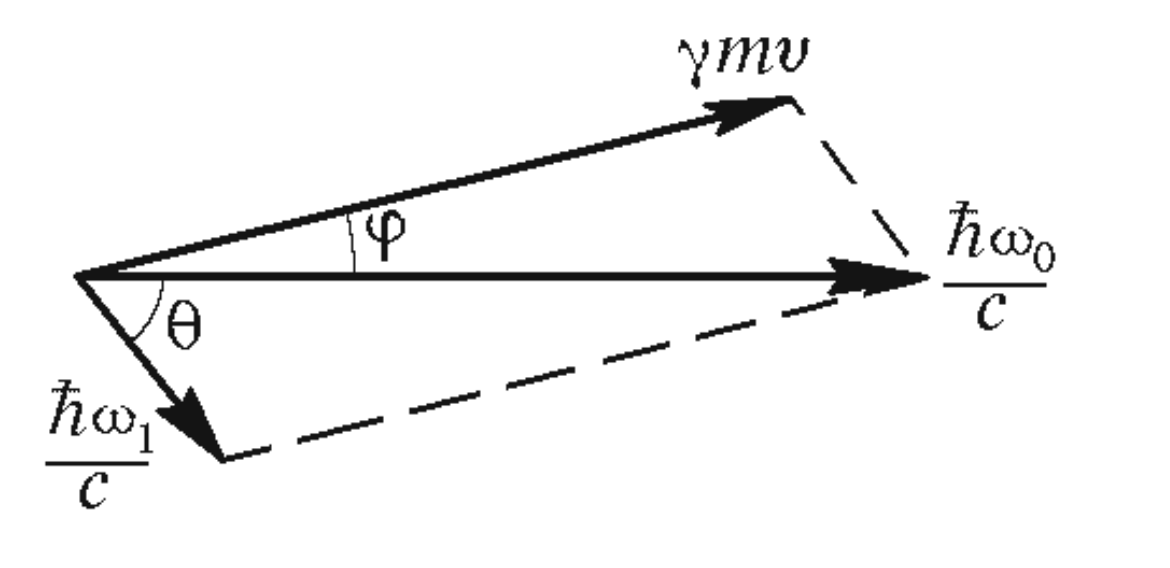
\includegraphics[scale = 0.2]{p1.png}
    \caption{Форма спектра $\beta$-частиц при разрешенных переходах}
    \label{p1}
\end{wrapfigure}

Запишем законы сохранения энергии и импульса:

$$mc^2 + \hbar\omega_0 = \gamma mc^2 + \hbar \omega_1$$
$$\frac{\hbar \omega_0}{c} = \gamma mv\cos{\phi} + \frac{\hbar \omega_1}{c}\cos{\theta}$$
$$\gamma mv\sin{\phi} = \frac{\hbar \omega_0}{c}\sin{\theta}$$

Перейдем от частот к длинам волн и получим изменение длины рассеяного света:

$$\Delta \lambda = \lambda_1 - \lambda_0 \frac{h}{mc} (1 - \cos{\theta})$$
$$\Lambda_k = \frac{h}{mc} = 2.42^{-10} \text{(см) - комптоновская длина волны электрона}$$

Перейдем от длин волн к энергии:

$$\frac{1}{\epsilon(\theta)} - \frac{1}{\epsilon_0} = 1 - \cos{\theta}$$

Здесь $\epsilon_0 = E_0 / (mc^2)$ - выраженная в единицах $mc^2$ энергия $\gamma$-квантов, 
падающих на рассеиватель, $\epsilon(\theta)$ - энергия квантов, испытавших комптоновское рассеяние на угол $\theta$.

\section{Экспериментальная установка}

Блок-схема установки изображена на рис.\ref{p2}. Источником излучения 1 служит $^{137}Cs$, испускающий $\gamma$-лучи с энергией 
662 кэВ. Он помещен в толстостенный контейнер с коллиматором. Сформированный коллиматором узкий пучок квантов подает на графитовую 
мишень 2.

\begin{figure}[h]
	\begin{center}
	\begin{minipage}[h]{0.5\linewidth}
	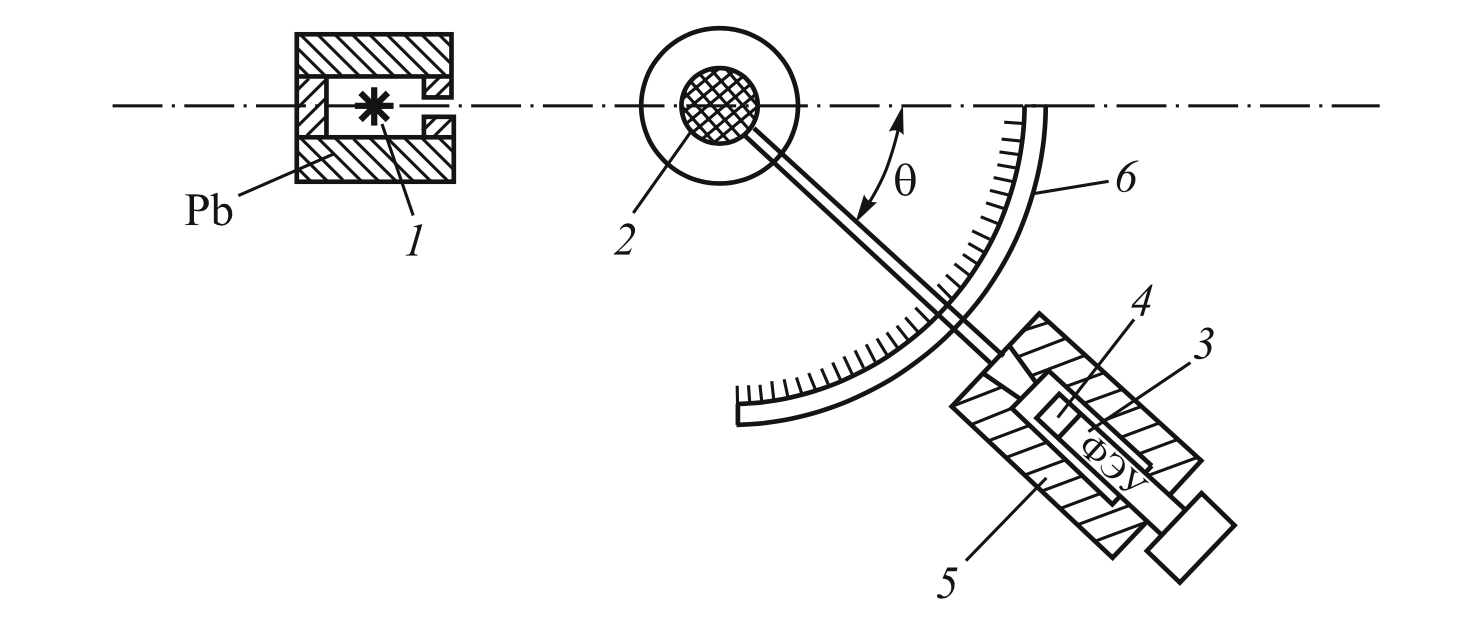
\includegraphics[width=1\linewidth]{p2.png}
	\caption{Блок схема установки} %% подпись к рисунку
	\label{p2} %% метка рисунка для ссылки на него
	\end{minipage}
	\hfill 
	\begin{minipage}[h]{0.3\linewidth}
	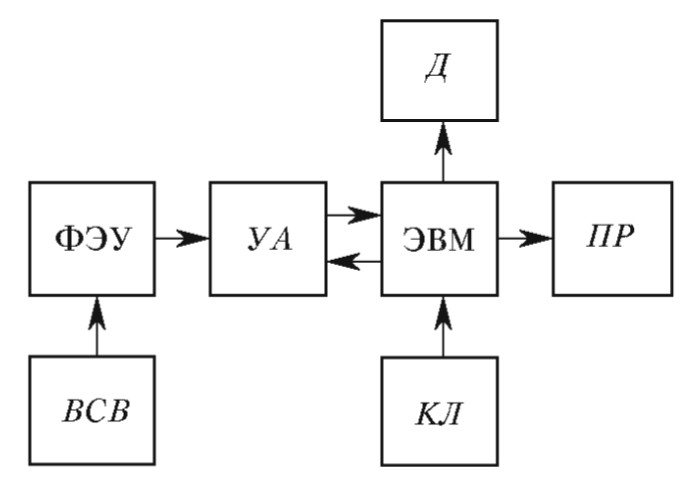
\includegraphics[width=1\linewidth]{p3.png}
	\caption{Блок-схема измерительного комлпекса}
	\label{p3}
	\end{minipage}
	\end{center}
\end{figure}

Кванты, испытавшие комптоновское рассеяние, регистрируются сцинтилляционным счетсчиком.
Он состоит из ФЭУ и сцинтиллятора. Сигналы, возникающие на аноде ФЭУ подаются на ЭВМ.

\section{Ход работы}

\begin{enumerate}
    \item Включим установку. Запустим программу и зайдем в режим измерения спектра.
    \item Устанавлиявая счетчик под разными углами от 0 до $120^{\circ}$ снимем спектры и занесем результат в таблицу \ref{table}

    \begin{table}[H]
        \centering
        \begin{center}
        \caption{Номер канала от угла наблюдения}
        \end{center}
        \vspace{0.1cm}
        \label{table}
        \begin{tabular}{ |c|c|c|c|c|c|c|c|c|c|c|c|c|c|}
    \hline
       Угол $\theta$,$^{\circ}$ & 0 & 10 & 20&30&40&50&60 \\
     \hline 
        N канала&774 $\pm$ 1&735 $\pm$ 1&649 $\pm$ 4&603 $\pm$ 2&529 $\pm$ 3&470 $\pm$ 3&433 $\pm$ 5\\
    \hline
       Угол $\theta$,$^{\circ}$ & 70&80&90&100&110&120& \\
     \hline 
        N канала&381 $\pm$ 2&343 $\pm$ 2&310 $\pm$ 3&275 $\pm$ 2&252 $\pm$ 3&234 $\pm$ 3&\\
    \hline
    \end{tabular}
    \end{table}

    \item Построим зависимость $1/N = f(1 - \cos{\theta})$:

    \begin{figure}[H]
        \begin{center}
        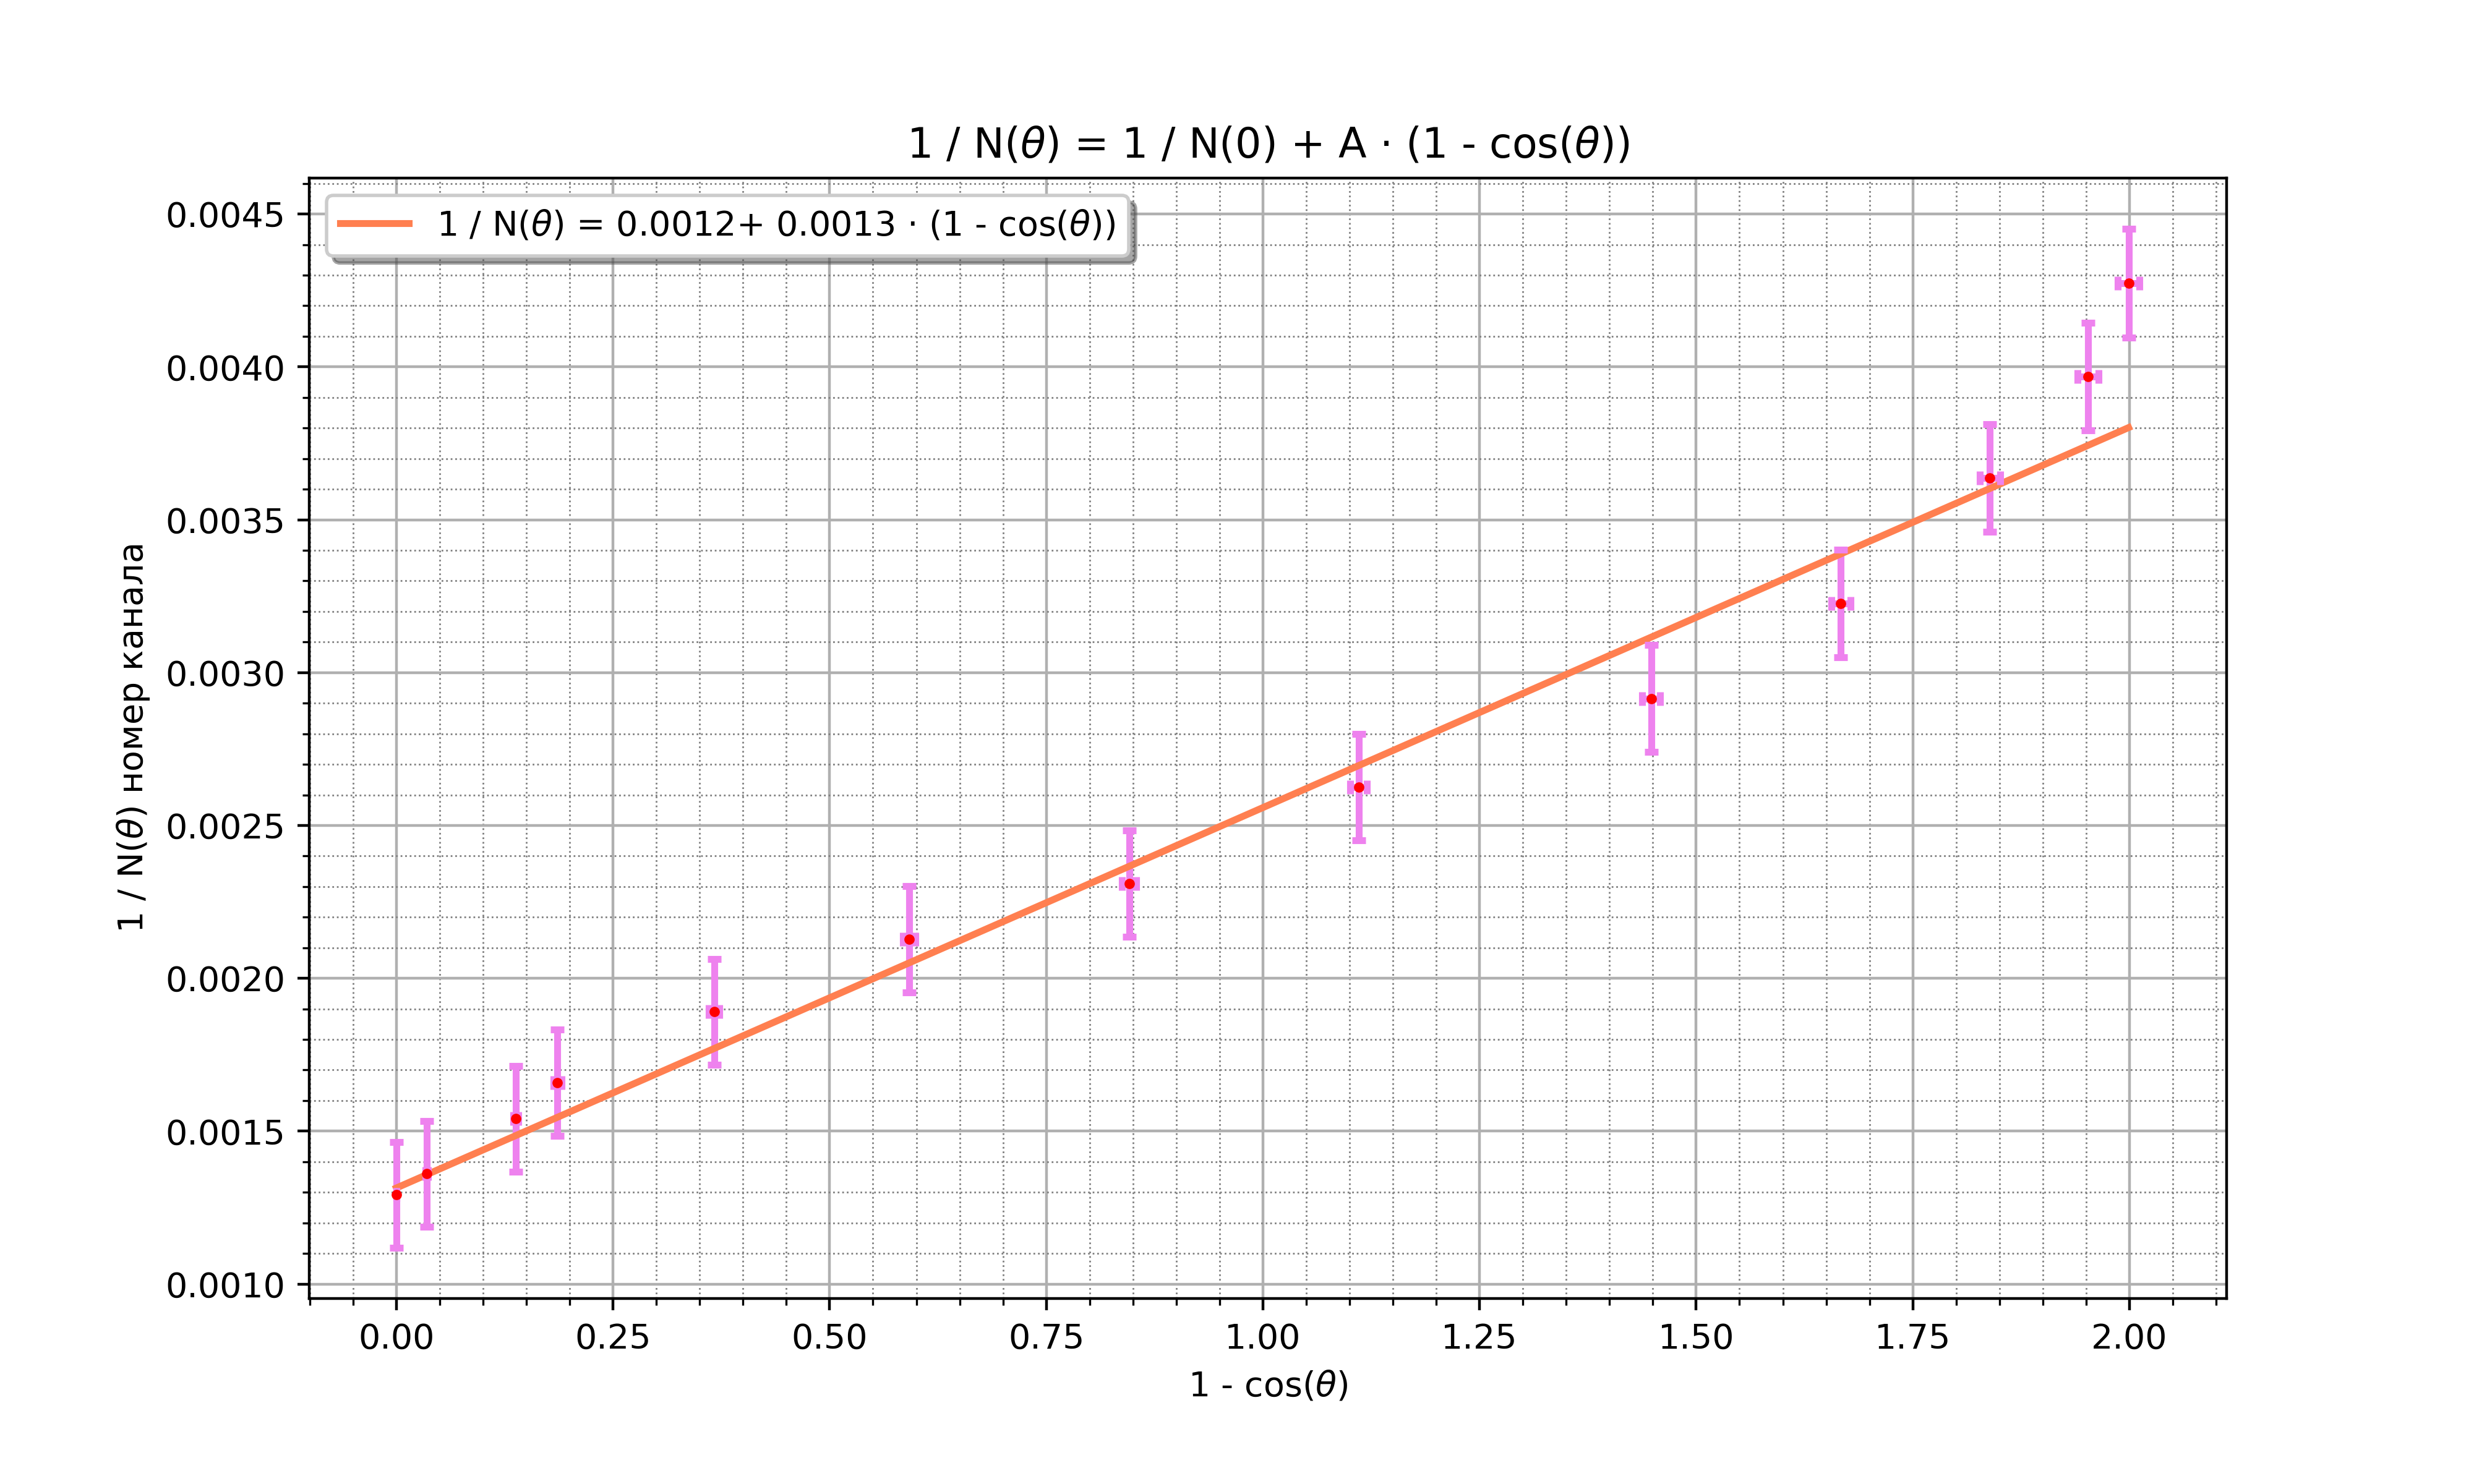
\includegraphics[scale = 0.6]{plot.png}
        \caption{График зависимости $1/N = f(1 - \cos{\theta})$}
        \label{plot}
        \end{center}
    \end{figure}

    Согласно формуле, точки ложатся на одну прямую. Пересечение этой прямой с осью 
    ординат опредлеяет наилучшее значение $N_{\text{наил}}(0)$. А пересечение линии с прямой $\cos{\theta} = 0$
    позволяет найти наилучшее значение $N_{\text{наил}}(90)$.

    Вернемся от переменной $\epsilon$ к энергии E, получим, что при $\theta = 90^{\circ}$ и формула 
    $\frac{1}{\epsilon(\theta)} - \frac{1}{\epsilon_0} = 1 - \cos{\theta}$ примет вид:
    $$mc^2 \left( \frac{1}{E(90)} - \frac{1}{E(0)} \right) = 1$$
    Или 
    $$mc^2 = E(0) \frac{E(90)}{E(0) - E(90)} = E_{\gamma} \frac{N(90)}{N(0) - N(90)}$$

    В этой формуле $E(0) = E_{\gamma}$ = 662кэВ - энергия электонов, рассеяных вперед. Номер канала, соответствующий фотопику,
    пропорционален энергии кванта. Значения N возьмем из графика, чтобы снизить случайную погрешность, полученную во время эксперимента
    (колебания напряжения сильно влияют на величину коэффициента усиления ФЭУ и эл. схем)

    Итак, согласно графику:

    $$N(90) = a + b = 391 \pm 16 , \;\;\;\; \sigma N(90) = \sqrt{\frac{\sigma_a}{ a}^2+\frac{\sigma_b}{b}^2}N(90) \;\;$$
    $$ N(0) = \frac{1}{b}= 791 \pm 12 ,\;\;\;\; \sigma N(0) = \frac{\sigma_b}{b} N(0) $$
    $$ a = (1,2 \pm 0,4)10^{-3},\; b = (1,3 \pm 0,2)10^{-3} $$
    Согласно выше выведенной формуле:

    $$mc^2 = 699  \pm 28 \text{кэВ},$$ где $$\sigma_{mc^2} = \sqrt{\frac{\sigma_a}{ a}^2+\frac{\sigma_b}{b}^2}mc^2\;\;$$


\end{enumerate}

\section{Вывод}

В ходе работы с помощью сцинтилляционного счетчика был измерен энергетический спектр $\gamma$-квантов,
рассеяных на графите. Проверен эффект Комптона, получена эксперементальная зависимость энергии рассеяния 
от угла наблюдения. Графическим способом получено значение энергии покоя электрона.


\end{document}